\chapter{Servizio di notifica}\label{service}

Il servizio di notifica implementato nell'applicazione utilizza RabbitMQ per raccogliere le informazione da trasmettere, genera il messaggio e poi lo spedisce mediante e-mail.\\
La struttura del microservizio è riportata di seguito:
\begin{flushleft}
\dirtree{%
.1 notificationservice.
.2 challenge.
.3 Challenge.java.
.3 ChallengeEventType.java.
.3 ChallengeResult.java.
.3 ChallengeStatus.java.
.2 mail.
.3 EmailService.java.
.3 EmailServiceConfig.java.
.3 SimpleMailMessageBuilder.java.
.2 messaging.
.3 Receiver.java.
.2 user.
.3 AppUser.java.
.3 UserPreference.java.
.3 UserPreferenceRepository.java.
.3 UserPreferenceService.java.
.2 AppConfig.java.
.2 Controller.java.
.2 NotificationServiceApplication.java.
}
\end{flushleft}

%%%%%%%%%%  PREFERENZE NOTIFICHE    %%%%%%%%%%
\section{Preferenze notifiche}

Nella web app vi è un'apposita sezione per le preferenze di notifica per avere un controllo granulare su quest'ultime. Come si può notare dalla figura \ref{fig:prefnot} vi sono vari campi dotati di check-box per poter selezionare quali notifiche ricevere.

\begin{figure}[H]
    \centering
    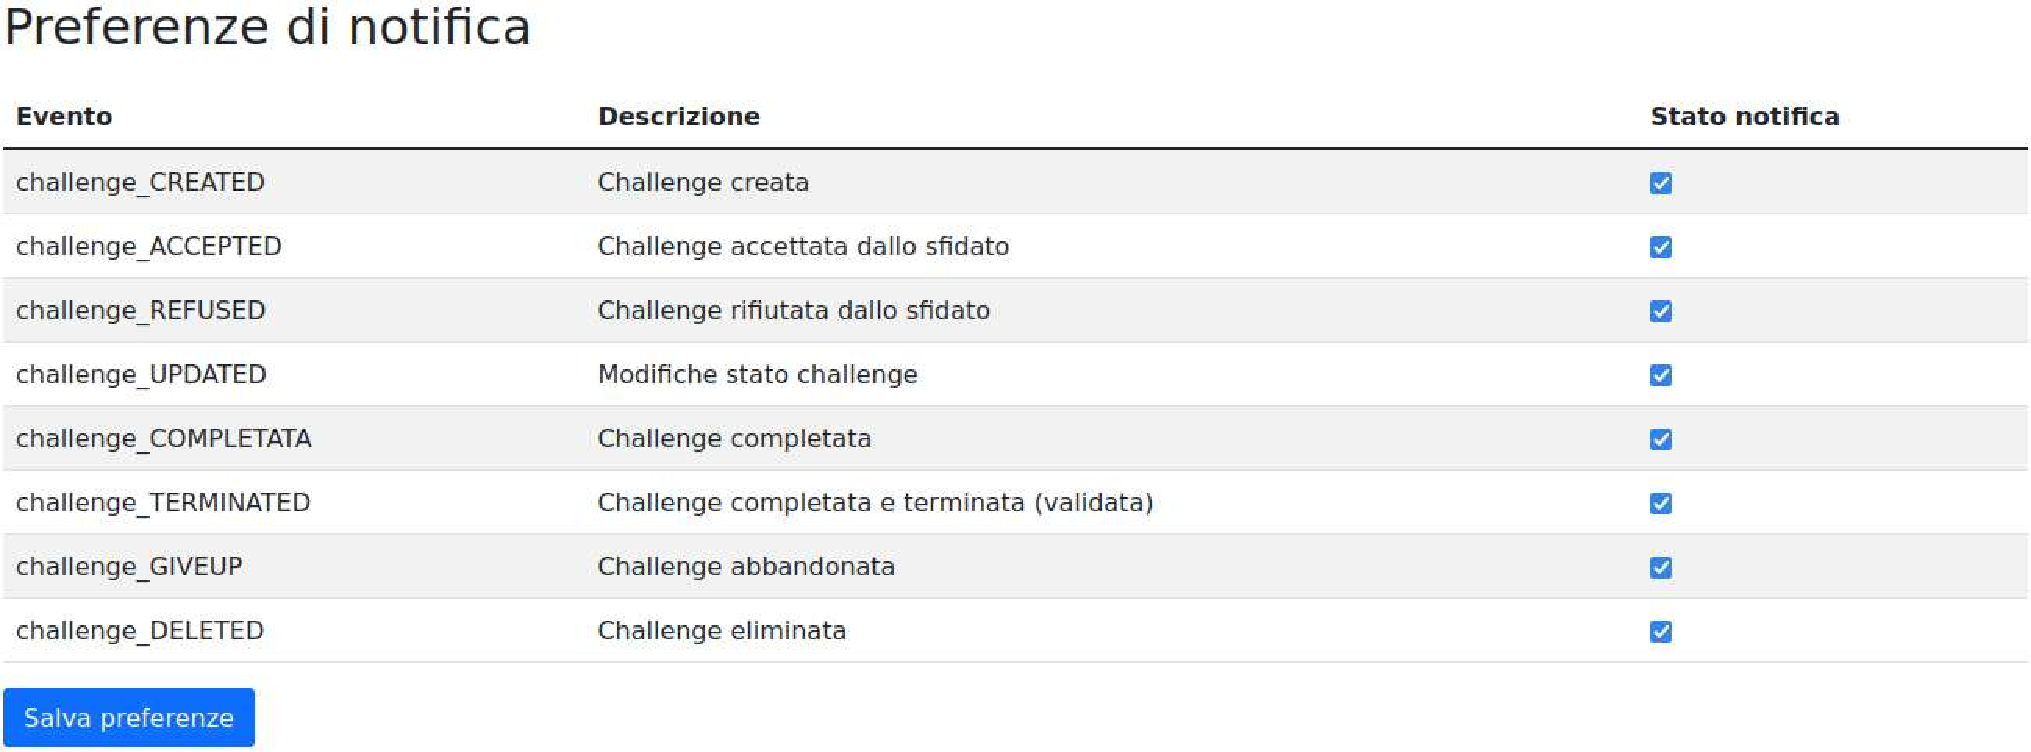
\includegraphics[width=1\textwidth]{images/preferenze-notifica.pdf}
    \caption{Preferenze di notifica webapp}
    \label{fig:prefnot}
\end{figure}

Al primo accesso si spuntano i check-box interessati e si salvano le proprie preferenze. Nel salvataggio viene creata una nuova istanza nella tabella \texttt{user\_preference}, contenente i campi scelti dall'utente, così da salvare il tutto permanentemente.

\begin{lstlisting}[language=Java, caption=Frammento codice preferenze utente, basicstyle=\footnotesize]
@Entity
public class UserPreference {
    @Id
    private Long userID;
    private boolean CHALLENGE_CREATED;
    private boolean CHALLENGE_ACCEPTED;
    private boolean CHALLENGE_REFUSED;
    private boolean CHALLENGE_COMPLETED;
    private boolean CHALLENGE_UPDATED;
    private boolean CHALLENGE_DELETED;
    private boolean CHALLENGE_GIVEUP;
    private boolean CHALLENGE_TERMINATED;
}
\end{lstlisting}

Come si può notare dal precedente frammento di codice, le istanze nel database hanno come \textit{primary key} l'id utente, mentre i rimanenti campi sono \texttt{boolean} dato che il dato contenuto è la preferenza dei check-box.\\
Dopo l'operazione di aggiornamento delle preferenze, durante il flusso dell'applicazione (utenti si sfidano, utenti completano le sfide, ..), verranno inviate ai rispettivi utenti le notifiche richieste: il mittente è \texttt{rabbitmailtest@gmail.com}, indirizzo creato appositamente per questa parte del progetto, l'oggetto sarà l'evento che ha scatenato l'invio dell'email ed il corpo del messaggio conterrà le informazioni specifiche, quali sfidato, sfidante, giudice, tempo di completamento, titolo e descrizione della sfida.

\begin{figure}[H]
    \centering
    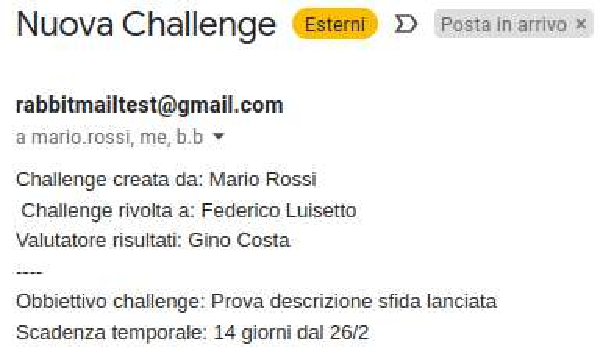
\includegraphics[width=9cm, height=5cm]{images/prova-email.pdf}
    \caption{Esempio mail}
\end{figure}

%%%%%%%%%%  GENERAZIONE MAIL   %%%%%%%%%%
\section{Generazione e-mail}

La generazione e l'invio delle e-mail sono gestiti dalla classe \texttt{EmailService}, appartenente alla sezione \textit{mail} del servizio. Quest'ultima delega la configurazione del servizio mail (protocollo, porta, nome utente, password, ...) a \texttt{EmailServiceConfig} e la costruzione della mail stessa (mittente, ricevitore, oggetto e corpo) a \texttt{SimpleMailMessageBuilder}
\begin{lstlisting}[language=Java, caption=Generazione corpo email, basicstyle=\footnotesize]
public void process(Challenge challenge, ChallengeEventType eventType)
{
    try {
        AppUser challenger = getUser(challenge.getChallenger());
        AppUser challenged = getUser(challenge.getChallenged());
        AppUser evaluator = getUser(challenge.getEvaluator());
        
        SimpleMailMessageBuilder mailBuilder = 
            new SimpleMailMessageBuilder(
            challenge,
            eventType,
            emailServiceConfig.username,
            challenger,
            challenged,
            evaluator);
        SimpleMailMessage message = mailBuilder.build();
        emailSender.send(message);
    } catch (Exception e) {
        e.printStackTrace();
    }
}
\end{lstlisting}

L'intero meccanismo di invio è messo in moto dalla classe \texttt{Receiver}, appartenente alla sezione \textit{messaging}, che mediante RabbitMQ si mette in ascolto dei nuovi messaggi nella coda \texttt{challengeQueue}. All'arrivo di un nuovo messaggio nella coda viene richiamato il metodo della classe \texttt{EmailService} sopra riportato.

\begin{lstlisting}[language=Java, caption=Ricezione update ed invio notifica, basicstyle=\footnotesize]
@EnableRabbit
@Service
public class Receiver {
    @Autowired
    EmailService emailService;
    static final public String queueName = "challengeQueue";
    @RabbitListener(queues = queueName)
    public void receiveMessage(byte[] newChallenge, 
        @Header(name="event_type") String eventType) {
    ObjectMapper mapper = new ObjectMapper();
    Challenge challenge = null;
    try {
      challenge = mapper.readValue(new String(newChallenge), 
        Challenge.class);
    } catch(JsonProcessingException e) {
      e.printStackTrace();
    }
    emailService.process(challenge, 
        ChallengeEventType.valueOf(eventType));
  }
}
\end{lstlisting}